\appendix


\chapter{Instructions for Use of the 950 Rotary Table on the Schaublin 13 Universal Milling Machine}

\section*{Main Features}

\begin{tabular}{@{}ll@{}}
    Table Diameter          & 250 mm      \\
    Total Height            & 90 mm       \\
    Inner Cone of the Table & Morse 2     \\
    Table Division          & Every 0° 1' \\
    Number of T-Slots       & 8           \\
\end{tabular}

\begin{figure}[h]
    \centering
    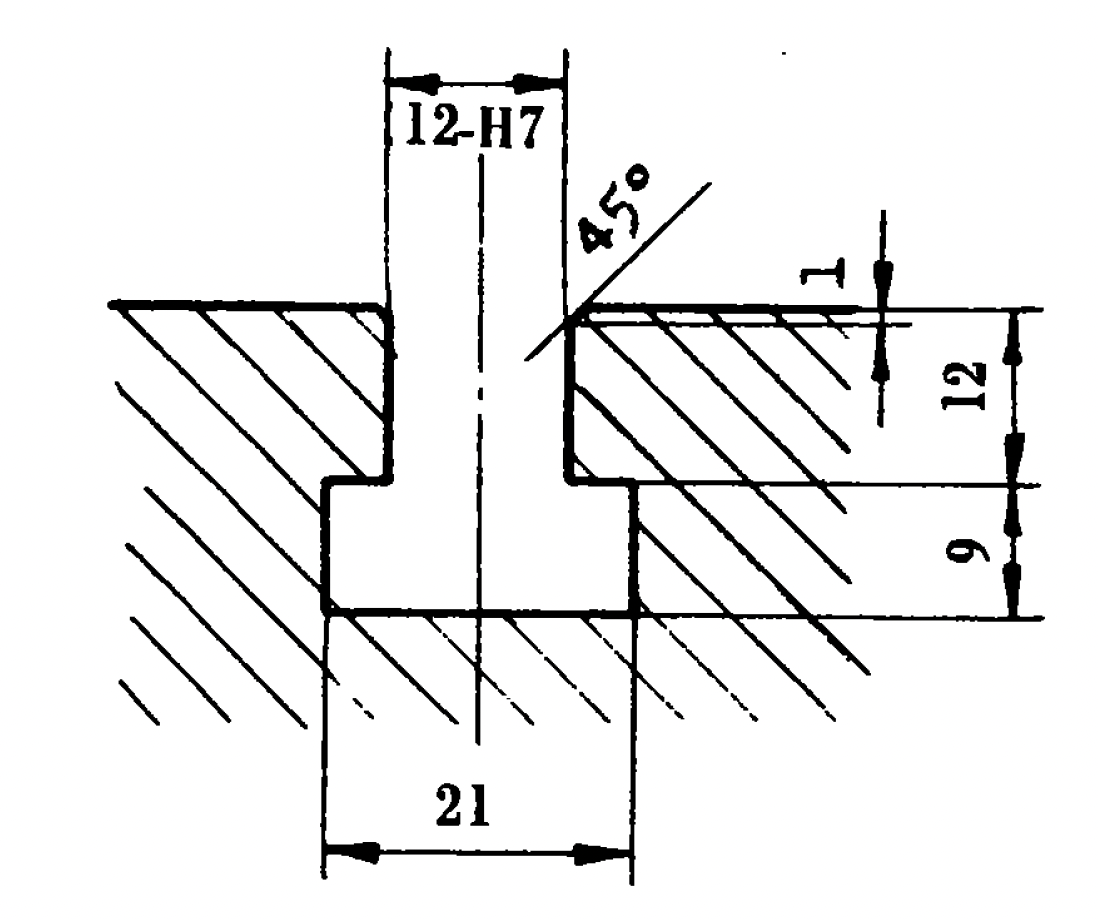
\includegraphics[width=0.6\linewidth]{images/rotary_table_t_slot_dimensions}
    \caption{T-Slot Dimensions \& According to VSM 33811}
    \label{fig:rotary_table_t_slot_dimensions}
\end{figure}


\section*{Accessory}

\begin{tabular}{@{}ll@{}}
    1050 & 3-disc dividing head with holes fitting on the rotary table. \\
    & Division: 2 to 360°                                          \\
    & \sout{Table of divisions: See IN 53-27 attached.}
\end{tabular}

\begin{notebox}
    Table of divisions is not included since online calculators can be used.\\
    The table has a 120:1 gear ratio.
    It comes with 3 plates with 15, 16, 17, 18, 19, 20, 21, 23, 27, 29, 31, 33, 37, 39, 41, 43, 47 and 49 holes.
\end{notebox}

The table is secured on two T-slots of the table using 4 bolts $\varnothing$10 provided with this accessory.
Two guide stones ensure its alignment on the table. Two eccentric locks immobilize the table.

To release the table from the worm, loosen screw 94 and turn eccentric sleeve 95 (see page 41). % TODO: add page reference
